\documentclass{article}
\usepackage{tgbonum}
\usepackage{graphicx}
\usepackage{fullpage}
\begin{document}
% Title Space
\title{Independent Study Proposal}
\author{Rahul Krishna}
\maketitle

% Abstract
\section{Abstract}
This independent study aims to explore the application of multidimensional 
prediction systems in predicting the defects in unseen data. The study proposes 
the use of contrast sets as a planner in order to help understand what changes 
are to be made to mitigate these defects. The efficacy of these changes will 
then be evaluated by using one of several established predictors, such as 
random forest, CART, logistic regression, and so on. The system consists of two 
phases-- Planning and Prediction. A flow chart of the proposed system is shown 
in Fig. \ref{fig1}. 

\begin{figure}[h!]
\centering
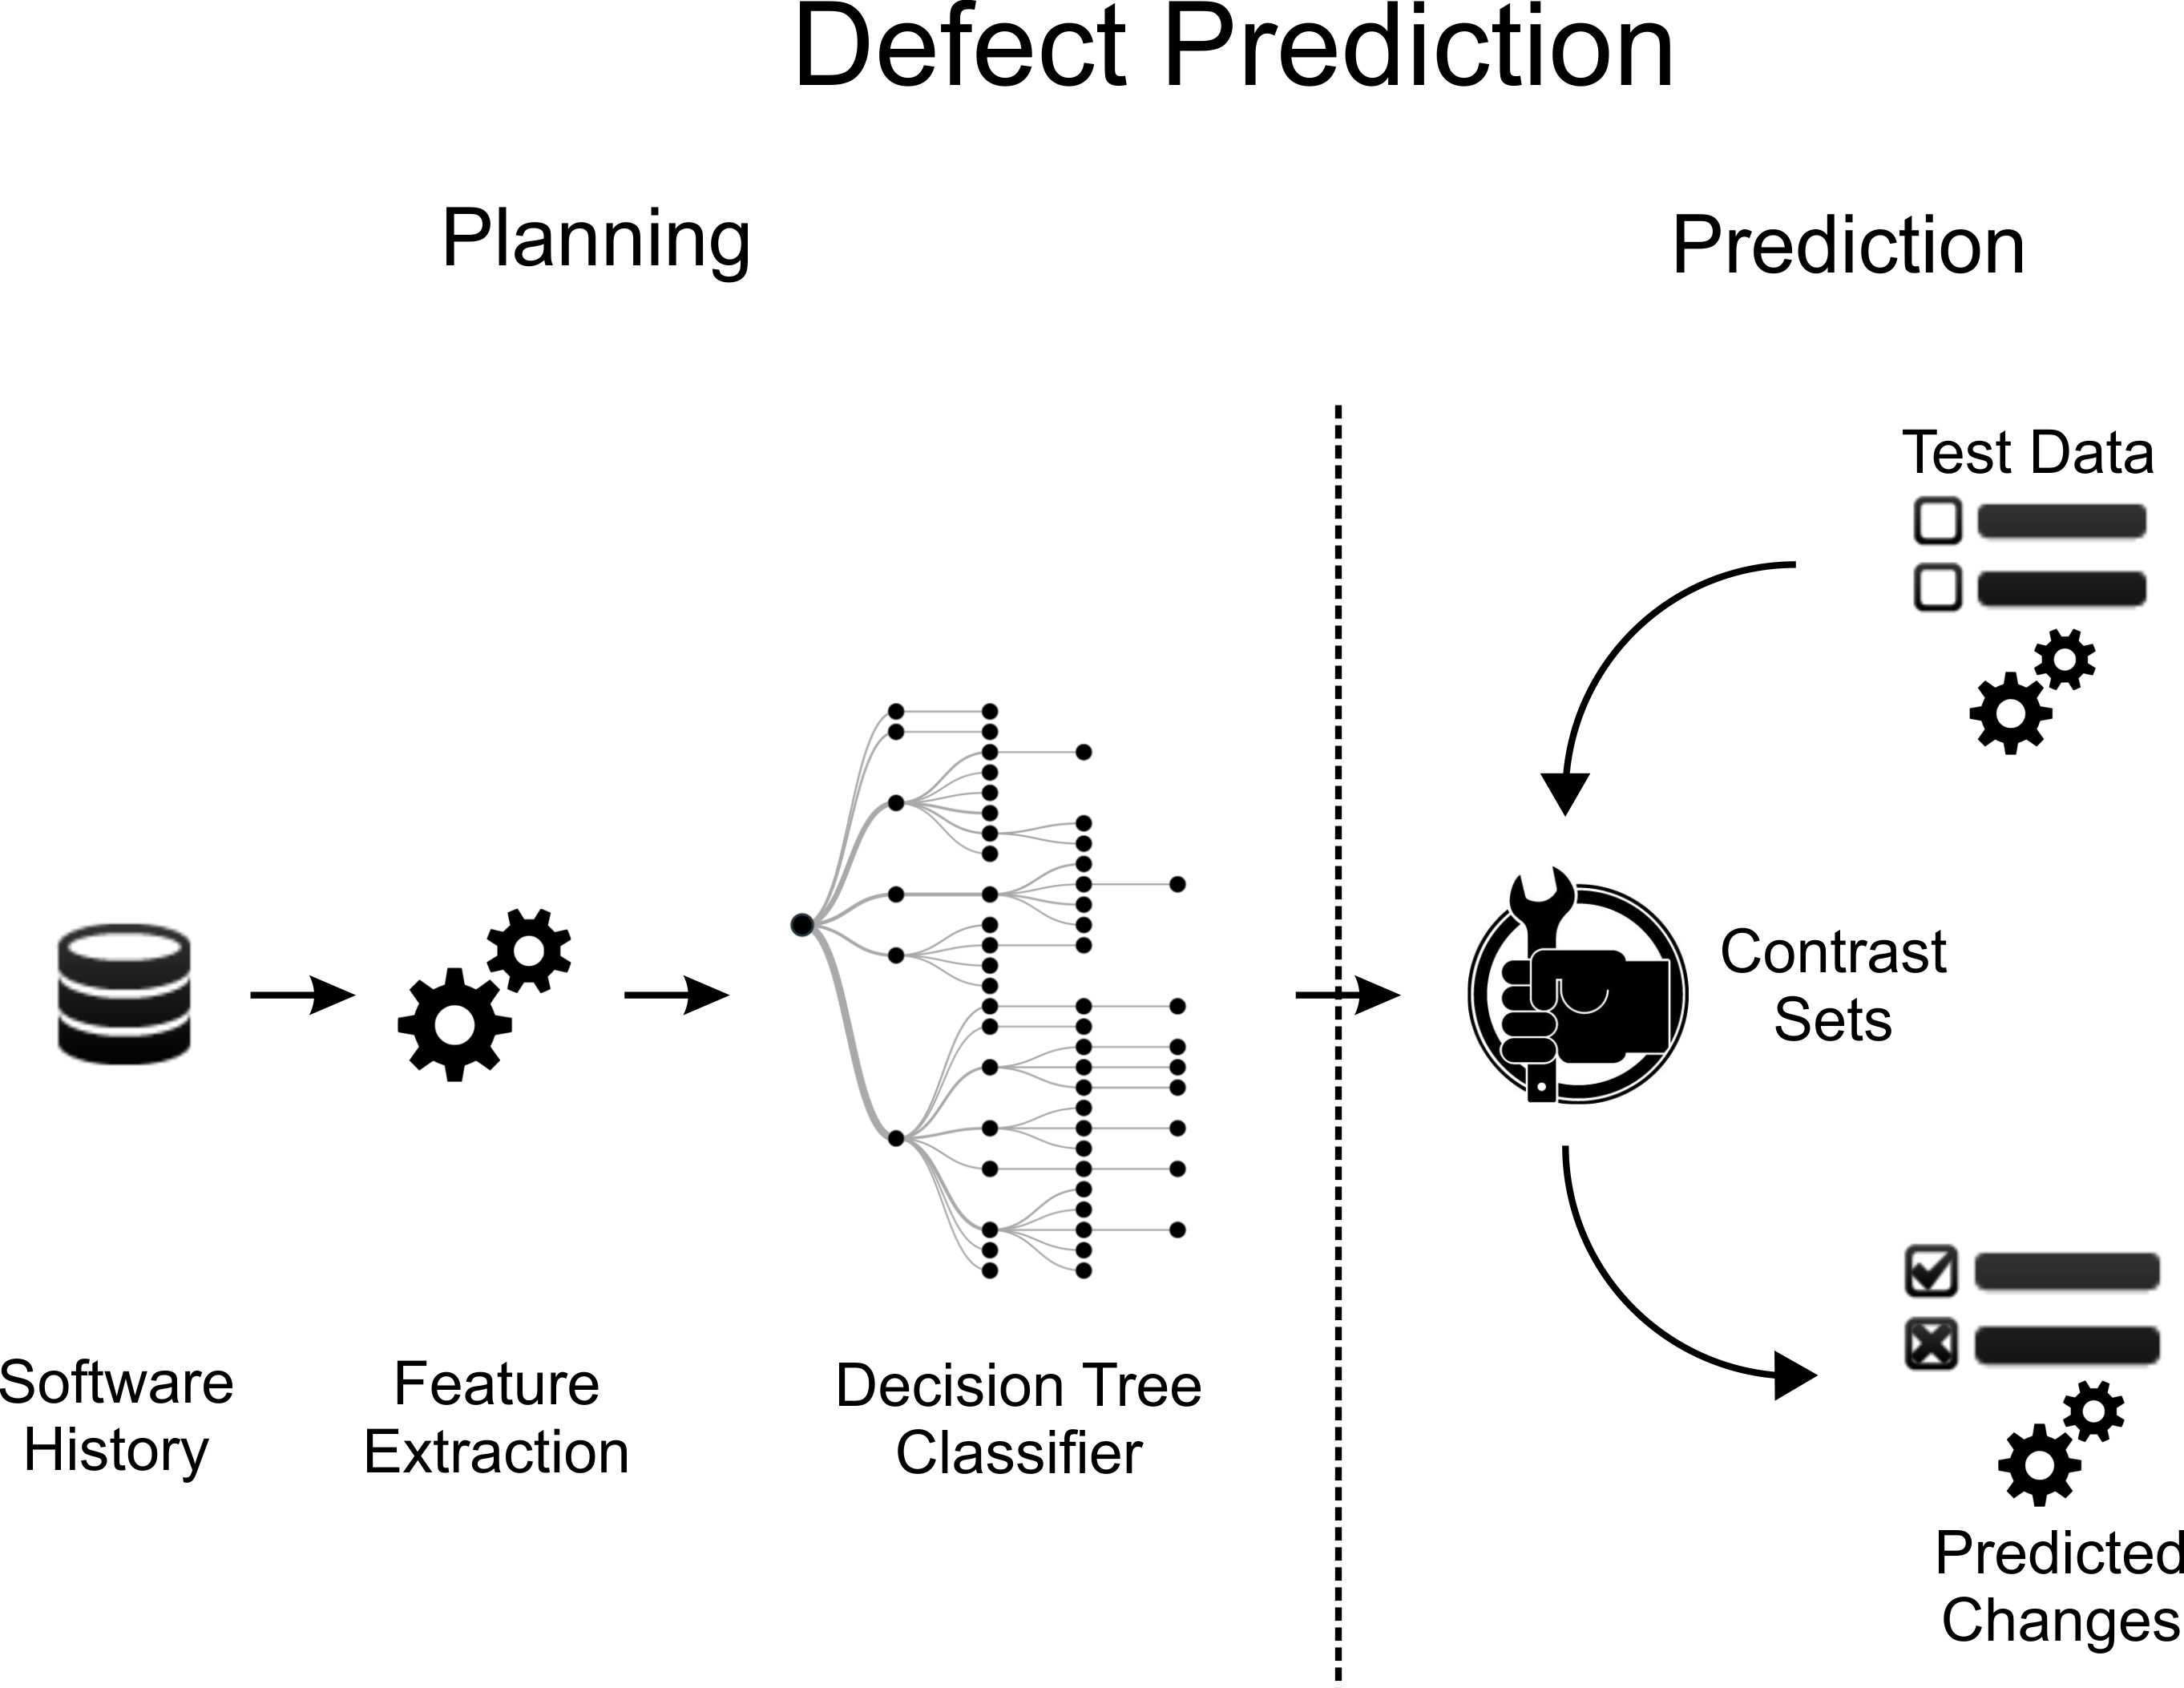
\includegraphics[width = 0.7\linewidth]{flowchart}
\caption{Flowchart of the proposed defect prediction system.}
\label{fig1}
\end{figure}

\noindent In the planning phase we use training data with recursive 
\textit{FASTMAP} clustering to create create clusters. For a test data, we 
generate contrast sets to indicate changes to be made to reduce defects. In the 
prediction phase, we implement these changes and 
\end{document}